% autore: Matilde Padovano

Questo problema, come si può facilmente notare, è greedy. Infatti parto da 0 con il primo taxi, ed a ogni città valuto quale tra il prezzo del taxi corrente aumentato di 1, e quello del nuovo taxi, è più basso, e proseguo con quello. Per ogni tratta sommo il costo del taxi su cui sto viaggiando al costo totale, e alla fine restituisco questa somma.\itemize

\colorbox{white}{\makebox[.99\textwidth][l]{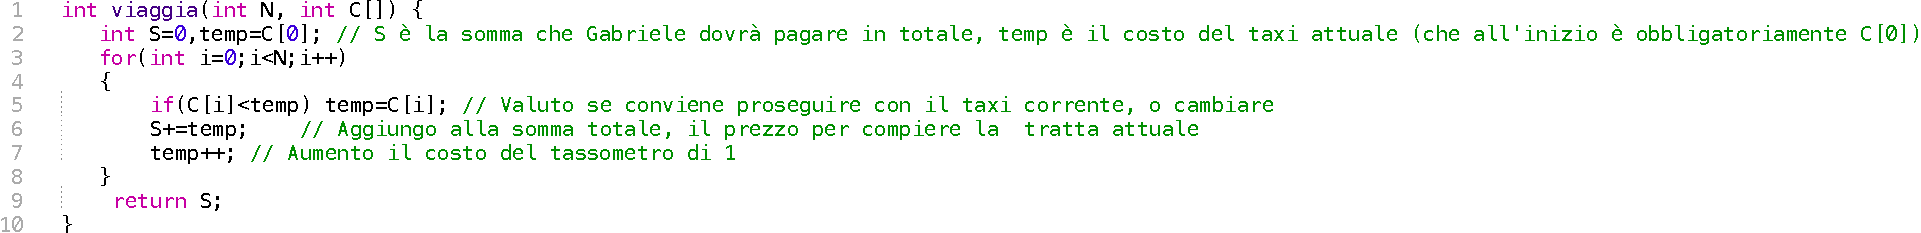
\includegraphics[scale=.8]{taxi.pdf}}} 